\input{head.inc}
  
% Präambelbefehle für die Präsentation
\title[TET: Elektromagnetische Wellen VI - Kugelwellen]{Elektromagnetische Wellen VI - Kugelwellen}

\begin{document}
% 
% Frontmatter 
% 
%%%%%%%%%%%%%%%%%%%%%%%%%%%%%%%%%%%%%%%%%%%%%%%%%%%%%%%%%%%%%%%%%%%%%%%%%%%%%%%%%%%%%%%%%%%%%%%%%%%%%%%%%%%%%%%%%%%%%%%%%%%%% 

%% inserts the title page and the table of contents
\maketitle

% 
% Content 
% 
%%%%%%%%%%%%%%%%%%%%%%%%%%%%%%%%%%%%%%%%%%%%%%%%%%%%%%%%%%%%%%%%%%%%%%%%%%%%%%%%%%%%%%%%%%%%%%%%%%%%%%%%%%%%%%%%%%%%%%%%%%%%% 
\section{Elektromagnetische Wellen VI - Kugelwellen}

\begin{frame}
  \frametitle{Ausgangspunkt}
  \begin{itemize}[<+->]
  \item Die bisher betrachteten \alert{ebenen Wellen} sind eine sehr wichtige Klasse der Lösungen der \alert{homogenen Wellengleichung}
    \begin{equation*}
      \square\Psi(\Ortsr[v],t) = \left(\laplace - \varepsilon\mu\frac{\d^2}{\d t^2}\right)\Psi(\Ortsr[v],t) = \left(\laplace - \frac{1}{\Geschwindigkeit_c^2}\frac{\d^2}{\d t^2}\right)\Psi(\Ortsr[v],t) = 0
    \end{equation*}
  \item Eine andere ebenso wichtige Klasse von Lösungen sind die \alert{Kugelwellen}.
  \item Diese werden genutzt (angesetzt), wenn eine \alert{kugelsymmetrische Lösung} dem Problem besser angepasst erscheint.
  \item Der \alert{Ansatz} ist dann:
    \begin{equation*}
      \boxed{\Psi(\Ortsr[v],t) \stackrel{!}{=} \Psi(\Ortsr,t)} \text{ mit } \Ortsr = |\Ortsr[v]|
    \end{equation*}
  \item Für den \alert{Laplace-Operator} in \alert{Kugelkoordinaten} \((r,\varphi,\vartheta)\) gilt dann:
    \begin{align*}
      \laplace \Psi &= \frac{1}{r} \frac{\d^2}{\d r^2}(r\Psi) + \frac{1}{r^2\sin\vartheta} \frac{\d}{\d\vartheta} \left(\sin\vartheta\frac{\d}{\d \vartheta}\right)\Psi + \frac{1}{r^2\sin^2\vartheta}\frac{\d^2}{\d \varphi^2}\Psi &\text{allgemein}\\
      \Aboxed{\laplace \Psi&= \frac{1}{r}\frac{\d^2}{\d r^2}(r\Psi)} & \Psi(\Ortsr[v],t) = \Psi(\Ortsr,t)
      \end{align*}
  \end{itemize}
  \end{frame}

\begin{frame}
  \frametitle{Einsetzen in die Wellengleichung}
  \begin{itemize}[<+->]
  \item Laplace Operator den für kugelsymmetrischen Fall
    \begin{equation*}
      \boxed{\laplace \Psi= \frac{1}{r}\frac{\d^2}{\d r^2}(r\Psi)} \text{ für } \Psi(\Ortsr[v],t) = \Psi(\Ortsr,t)
    \end{equation*}
  \item Einsetzen in die Wellengleichung ergibt:
    \begin{align*}
      \laplace \Psi(\Ortsr,t) - \frac{1}{\Geschwindigkeit_c^2}\frac{\d^2}{\d t^2}\Psi(\Ortsr,t) &= 0\\
      \frac{1}{r}\frac{\d^2}{\d r^2}(r\Psi(\Ortsr,t)) - \frac{1}{\Geschwindigkeit_c^2}\frac{\d^2}{\d t^2}\Psi(\Ortsr,t) &= 0\\
      \ergo \Aboxed{\left(\frac{\d^2}{\d r^2} - \frac{1}{\Geschwindigkeit_c^2}\frac{\d^2}{\d t^2}\right)(r\Psi(\Ortsr,t)) &= 0} 
    \end{align*}
    \item Die Funktion \alert{\(r\Psi(\Ortsr,t)\)} ist somit Lösung der homogenen eindimensionalen Wellengleichung! \(\to\) Bekannt aus Block \alert{Ebene Wellen}.
  \end{itemize}
  \end{frame}

\begin{frame}
  \frametitle{Kugelwellen}
  \begin{itemize}[<+->]
  \item Offenbar kann \(r\Psi(\Ortsr,t)\) dann als Überlagerung der Funktionen \(\Psi_+\) und \(\Psi_-\) geschrieben werden:
    \begin{align*}
      r\Psi(\Ortsr, t) &= \Psi_+(\omega t + \Wellenzahl r) + \Psi_-(\omega t - \Wellenzahl r) \text{ mit } \omega=\Wellenzahl \Geschwindigkeit_p \; (\omega \ge 0)\\
      \ergo \Aboxed{\Psi(\Ortsr, t) &= \frac{1}{r} \left(\Psi_+(\omega t + \Wellenzahl r) + \Psi_-(\omega t - \Wellenzahl r)\right)} \\
      & \Psi_+(\omega t + \Wellenzahl r)  \text{ einlaufende Welle}\\
      & \Psi_-(\omega t - \Wellenzahl r)  \text{ auslaufende Welle}
    \end{align*}
  \item Wir haben damit eine \alert{neue Klasse} von Lösungen gefunden. Die Eigenschaften sind:
    \begin{enumerate}[<+->]
    \item Phase: \(\varphi_\pm = \omega t \pm kr \to \) nur abhängig von \(\Ortsr =|\Ortsr[v]| \Rightarrow \) \alert{Die Phasenflächen sind Kugelflächen}
    \item Amplitude: \(\propto \dfrac{1}{\Ortsr}\)
    \item Für \alert{harmonische Zeitabhängigkeit}: \(\underline{\Psi}_\pm = \dfrac{1}{r}\underline{A}_\pm\euler^{\komplex(\omega t \pm kr)}\) \ergo Kugelwellen im engeren Sinne
    \item Phasengeschwindigkeit: \(\Geschwindigkeit_p = \mp \dfrac{\omega}{k} = \mp \dfrac{c}{n} =\Geschwindigkeit_c\)
      \item Abstand von Flächen gleicher Phase (Wellenlänge): \(\Wellenzahl \lambda = 2\pi\)
      \end{enumerate}
    \end{itemize}
    \ 
  \end{frame}

\begin{frame}
  \frametitle{Kugelwellen -- Visualisierung}
  \centering\includegraphics[width=\textwidth]{kugelwelle}
  \begin{columns}
    \begin{column}{0.5\textwidth}
      \centerline{Ebene durch Ursprung}
      \begin{itemize}
      \item Divergenz bei \(r=0\) ausgeblendet
      \item Phasenflächen = Kugelschalen
        \item hier: nur auslaufende Lösung
        \end{itemize}
    \end{column}
    \begin{column}{0.5\textwidth}
      \centerline{Amplitude entlang Radialrichtung}
      \begin{itemize}
      \item Einhüllende \(\propto \nicefrac{1}{r}\)
        \item hier: \(\Geschwindigkeit_p = c \to \SI{1}{\nano\second} \simeq \SI{33}{\centi\meter}\)
      \item Bisher nur eine Größe; z.B. nur E-Feld 
        \end{itemize}
      \end{column}
    \end{columns}
  \end{frame}
    
\begin{frame}
  \frametitle{Betrachtung der Felder}
  \begin{itemize}[<+->]
  \item Formal haben Lösungen der homogenen Wellengleichung für elektrisches Feld und magnetische Flussdichte die \alert{gleiche Form}.
  \item Aber natürlich sind die Größen weiterhin über die Maxwell-Gleichungen miteinander \alert{verkoppelt}
  \item Es sind \(\EFeld[uv]\) und \(\BFeld[uv]\) gegeben durch
    \begin{equation*}
      \EFeld[uv](\Ortsr, t) = \EFeld[uv]_0 \frac{1}{r} \euler^{\komplex(\omega t - kr)} \text{ und } \BFeld[uv](\Ortsr, t) = \BFeld[uv]_0 \frac{1}{r} \euler^{\komplex(\omega t - kr)}
    \end{equation*}
  \item Dann folgt wegen \(\divergenz \EFeld[uv] = 0\) und \(\divergenz\BFeld[uv]=0\) z.B. für das elektrische Feld:
     \begin{align*}
      \divergenz \EFeld[uv]  & = \frac{1}{r^2} \frac{\d}{\d r} \left( r^2 \EFeld[uv]_0 \frac{1}{r} \euler^{\komplex(\omega t -kr)} \right) \cdot \einheitsvek{r} \quad\to\text{Was passiert mit den anderen Summanden?}\\
                             &= \left( \EFeld[uv]_0 \cdot \einheitsvek{r} \right) \frac{1}{r^2} \euler^{\komplex(\omega t -kr)} \left(1- \komplex kr \right) \stackrel{!}{=} 0 \text{ für alle } k \text{ und } r  \\
       \Rightarrow \quad & \boxed{\EFeld[v] \perp \Ortsr[v]} \text{ und analog } \boxed{\BFeld[v] \perp \Ortsr[v]} \Rightarrow \text{ \alert{beide transversal!}}
       \end{align*}
     \end{itemize}
  \end{frame}

\begin{frame}
  \frametitle{Betrachtung der Felder (\dots)}
  \begin{itemize}[<+->]
  \item Wir nutzen das Induktionsgesetz
    \begin{equation*}
      \rotation \EFeld[v] = -\dfrac{\d}{\d t}\BFeld[v] \text{ bzw. } -\komplex \Wellenzahl \left(\einheitsvek{r} \times \EFeld[uv] \right) = -\komplex \omega \BFeld[uv]
    \end{equation*}
  \item Hiermit folgt unmittelbar, dass es sich (lokal) wieder um eine \alert{TEM-Welle} handelt:
    \begin{equation*}
      \BFeld[v] = - \frac{\Wellenzahl}{\omega} \left(\EFeld[uv] \times \einheitsvek{r} \right) = - \frac{1}{\Geschwindigkeit_p} \left(\EFeld[uv] \times \einheitsvek{r} \right) = - \frac{1}{\Geschwindigkeit_p} \left(\EFeld[uv] \times \einheitsvek{k} \right)  \quad \raisebox{-.5cm}{\kartkoordinatensystem[2]{\BFeld[v]}{\Wellenzahl[v]}{\EFeld[v]}}
    \end{equation*}
  \item Für viele Anwendungen wichtig ist der \alert{Wellenwiderstand}:
    \begin{equation*}
      \boxed{\underline{Z} = \frac{\EFeld[u]_0}{\HFeld[u]_0} = \frac{\mu \EFeld[u]_0}{\BFeld[u]_0} = \mu\Geschwindigkeit_p  = \mu \Geschwindigkeit_c= \sqrt{\frac{\mu}{\varepsilon}}} \quad \text{ hier: reel; allgemein: komplex}
    \end{equation*}
    \item \alert{Wellenwiderstand des Vakuums:} \(\boxed{Z_0 = \sqrt{\dfrac{\mu_0}{\varepsilon_0}} =\mu_0c\simeq \SI{120\pi}{\ohm} \simeq \SI{377}{\ohm}}\)
    \end{itemize}
    \ 
  \end{frame}


\begin{frame}
  \frametitle{TE und TM-Wellen}
  \begin{itemize}[<+->]
  \item Ebene Wellen, Kugelwellen: TEM-Wellen \(\to\) Aber das ist nicht immer so!
  \item Betrachten nun: Überlagerung zweier ebener Wellen gleicher Frequenz, Amplitude und Phasenlage, die sich in \alert{unterschiedlicher Richtung} ausbreiten.
  \begin{columns}
    \begin{column}{.35\textwidth}
  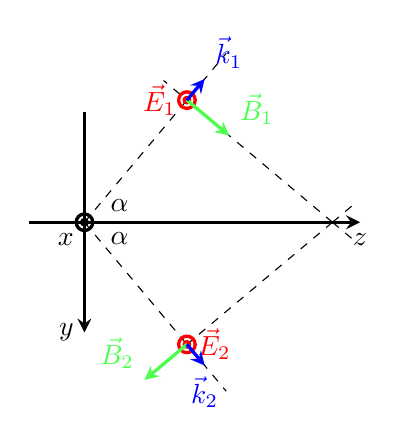
\begin{tikzpicture}[line width = 1.2pt, line join=round,>=stealth,scale=.7]
\draw [->] (-1,0,0) -- (5,0,0) node[anchor=north] {$z$};
\draw [->] (0,2,0) -- (0,-2,0) node[anchor=east] {$y$};
\draw (0,0) circle (1.5 mm); 
\draw (0,0) circle (.5 mm) node[anchor=north east]{$x$}; 

\draw[thin,dashed] (0,0) -- (50:4); 
\draw[thin,dashed] (0,0) -- (-50:4); 

\draw[thin,dashed] (4.5,0) -- +(140:4); 
\draw[thin,dashed] (4.5,0) -- +(-140:4); 
\draw[thin,dashed] (4.5,0) -- +(-40:.5); 
\draw[thin,dashed] (4.5,0) -- +(40:.5); 

\centerarc[thin,dotted](0,0)(0:50:1);
\node at (25:0.7) {$\alpha$};
\centerarc[thin,dotted](0,0)(0:-50:1);
\node at (-25:0.7) {$\alpha$};

\draw[red] (1.859,2.216) circle (1.5 mm); 
\draw[red] (1.859,2.216) circle (.5 mm) node[anchor=east]{$\vec{E}_1$};
\draw[green!70, ->] (1.859,2.216) -- +(-40:1) node[anchor=south west]{$\vec{B}_1$};
\draw[blue, ->] (1.859,2.216) -- +(50:.5) node[anchor=south west]{$\vec{k}_1$};

\draw[red] (1.859,-2.216) circle (1.5 mm); 
\draw[red] (1.859,-2.216) circle (.5 mm) node[anchor=west]{$\vec{E}_2$}; 
\draw[green!70, ->] (1.859,-2.216) -- +(-140:1) node[anchor=south east]{$\vec{B}_2$};
\draw[blue, ->] (1.859,-2.216) -- +(-50:.5) node[anchor=north]{$\vec{k}_2$};

\end{tikzpicture}
\end{column}
\begin{column}{.65\textwidth}
  \begin{itemize}[<+->]
  \item \(\EFeld[uv]_1 = \EFeld[uv]_0 \euler^{\komplex (\omega t - \Wellenzahl[v]_1\cdot\Ortsr[v])} = \EFeld[u]_{0} \einheitsvek{x} \euler^{\komplex (\omega t - \Wellenzahl[v]_1\cdot\Ortsr[v])}\) und
    \( \BFeld[uv]_1 = \dfrac{\Wellenzahl[v]}{\omega}\times\EFeld[uv]_1=\dfrac{1}{\Geschwindigkeit_p} \left( \einheitsvek{k_1} \times \EFeld[uv]_0 \euler^{-\komplex \Wellenzahl[v]_1\cdot\Ortsr[v]}\right) \euler^{\komplex \omega t }\)
  \item \(\EFeld[uv]_2 = \EFeld[uv]_0 \euler^{\komplex (\omega t - \Wellenzahl[v]_2\cdot\Ortsr[v])} = \EFeld[u]_{0}\einheitsvek{x}\euler^{\komplex (\omega t - \Wellenzahl[v]_2\cdot\Ortsr[v])}\) und
    \( \BFeld[uv]_2 = \dfrac{\Wellenzahl[v]}{\omega}\times\EFeld[uv]_2=\dfrac{1}{\Geschwindigkeit_p} \left( \einheitsvek{k_2} \times \EFeld[uv]_0 \euler^{-\komplex \Wellenzahl[v]_2\cdot\Ortsr[v]}\right) \euler^{\komplex \omega t }\)
  \item \( \Wellenzahl[v]_1 = -\Wellenzahl_y\einheitsvek{y} + \Wellenzahl_z\einheitsvek{z}  \) und \( \Wellenzahl[v]_2 = \Wellenzahl_y\einheitsvek{y} + \Wellenzahl_z\einheitsvek{z}  \)
  \item \alert{Überlagerung} der beiden Wellen:
    \begin{align*}
      \EFeld[uv] &= 2\EFeld[u]_{0}\cos(\Wellenzahl_yy) \einheitsvek{x} \euler^{\komplex(\omega t - \Wellenzahl_z z)} \\
      \BFeld[uv] &= \frac{2\EFeld[u]_{0}}{\Wellenzahl \Geschwindigkeit_p} \left( \Wellenzahl_z \cos(\Wellenzahl_y y) \einheitsvek{y} + \komplex \Wellenzahl_y\sin(\Wellenzahl_y y) \einheitsvek{z}\right) \euler^{\komplex(\omega t - \Wellenzahl_z z)}
    \end{align*}
  \item \alert{TE-Welle}, Propagation in z-Richtung (H-Wellen) \\
    analog: \alert{TM-Wellen} (E-Welle)
    \end{itemize}
\end{column}
\end{columns}
\end{itemize}
\ 
\end{frame}


\begin{frame}
  \frametitle{TE und TM-Wellen -- Phasengeschwindigkeit}
  \begin{itemize}[<+->]
  \item Phasengeschwindigkeit: \( \Geschwindigkeit_p = \dfrac{\omega}{\Wellenzahl_z}\); \(\Wellenzahl_z\) weil Ausbreitung in z-Richtung
  \item Für die einzelnen Wellen gilt \(\Geschwindigkeit_c = \dfrac{\omega}{\Wellenzahl} = \dfrac{\omega}{\sqrt{\Wellenzahl_y^2+\Wellenzahl_z^2}} \Rightarrow \Wellenzahl_z = \sqrt{\dfrac{\omega^2}{\Geschwindigkeit_c^2}-\Wellenzahl_y^2 }\)
  \item Hiermit folgt für die Phasengeschwindigkeit:
    \begin{align*}
      \Geschwindigkeit_p & = \frac{\omega}{\Wellenzahl_z} = \frac{\omega}{\sqrt{\frac{\omega^2}{\Geschwindigkeit_c^2}-\Wellenzahl_y^2 }} \\
                & = \frac{\omega}{\frac{\omega}{\Geschwindigkeit_c}\sqrt{1-\frac{\Wellenzahl_y^2 \Geschwindigkeit_c^2}{\omega^2} }} = \frac{\Geschwindigkeit_c}{\sqrt{1-\frac{\Wellenzahl_y^2 \Geschwindigkeit_c^2}{\omega^2} }} \ge \Geschwindigkeit_c 
      \end{align*}
    \item Die Phasengeschwindigkeit ist hier also mindestens so groß wie die Ausbreitungsgeschwindigkeit im Medium
    \item Im Vakuum kann die Phasengeschwindigkeit somit \alert{größer als die Lichtgeschwindigkeit} sein!
      \item Mehr zu TE- und TM-Wellen \(\to\) \alert{Hohlleiter} 
    \end{itemize}
\end{frame}
  
\input{finalframe.inc}
   
\end{document}